\documentclass[twoside,11pt]{article}

% ? Specify used packages
\usepackage{graphicx}        %  Use this one for final production.
% \usepackage[draft]{graphicx} %  Use this one for drafting.
% ? End of specify used packages

\pagestyle{myheadings}

% -----------------------------------------------------------------------------
% ? Document identification
\newcommand{\stardoccategory}  {Starlink Guide}
\newcommand{\stardocinitials}  {SG}
\newcommand{\stardocsource}    {sg\stardocnumber}
\newcommand{\stardocnumber}    {10.2}
\newcommand{\stardocauthors}   {Grant Privett}
\newcommand{\stardocdate}      {30 January 1998}
\newcommand{\stardoctitle}     {Preparing to Observe}
\newcommand{\stardocversion}   {Software and WWW-Based Resources}
\newcommand{\stardocmanual}    { }
\newcommand{\stardocabstract}  {This document identifies a number of software
applications and packages that will prove useful to observers writing an
observing application or preparing for an observing run.
A brief description of the software is given.

WWW URLs are provided for WWW-based resources such a databases, catalogues and on-line atlases.
}

% ? End of document identification

% -----------------------------------------------------------------------------

\newcommand{\stardocname}{\stardocinitials /\stardocnumber}
\markboth{\stardocname}{\stardocname}
\setlength{\textwidth}{160mm}
\setlength{\textheight}{230mm}
\setlength{\topmargin}{-2mm}
\setlength{\oddsidemargin}{0mm}
\setlength{\evensidemargin}{0mm}
\setlength{\parindent}{0mm}
\setlength{\parskip}{\medskipamount}
\setlength{\unitlength}{1mm}

% -----------------------------------------------------------------------------
%  Hypertext definitions.
%  ======================
%  These are used by the LaTeX2HTML translator in conjunction with star2html.

%  Comment.sty: version 2.0, 19 June 1992
%  Selectively in/exclude pieces of text.
%
%  Author
%    Victor Eijkhout                                      <eijkhout@cs.utk.edu>
%    Department of Computer Science
%    University Tennessee at Knoxville
%    104 Ayres Hall
%    Knoxville, TN 37996
%    USA

%  Do not remove the %begin{latexonly} and %end{latexonly} lines (used by
%  star2html to signify raw TeX that latex2html cannot process).
%begin{latexonly}
\makeatletter
\def\makeinnocent#1{\catcode`#1=12 }
\def\csarg#1#2{\expandafter#1\csname#2\endcsname}

\def\ThrowAwayComment#1{\begingroup
    \def\CurrentComment{#1}%
    \let\do\makeinnocent \dospecials
    \makeinnocent\^^L% and whatever other special cases
    \endlinechar`\^^M \catcode`\^^M=12 \xComment}
{\catcode`\^^M=12 \endlinechar=-1 %
 \gdef\xComment#1^^M{\def\test{#1}
      \csarg\ifx{PlainEnd\CurrentComment Test}\test
          \let\html@next\endgroup
      \else \csarg\ifx{LaLaEnd\CurrentComment Test}\test
            \edef\html@next{\endgroup\noexpand\end{\CurrentComment}}
      \else \let\html@next\xComment
      \fi \fi \html@next}
}
\makeatother

\def\includecomment
 #1{\expandafter\def\csname#1\endcsname{}%
    \expandafter\def\csname end#1\endcsname{}}
\def\excludecomment
 #1{\expandafter\def\csname#1\endcsname{\ThrowAwayComment{#1}}%
    {\escapechar=-1\relax
     \csarg\xdef{PlainEnd#1Test}{\string\\end#1}%
     \csarg\xdef{LaLaEnd#1Test}{\string\\end\string\{#1\string\}}%
    }}

%  Define environments that ignore their contents.
\excludecomment{comment}
\excludecomment{rawhtml}
\excludecomment{htmlonly}

%  Hypertext commands etc. This is a condensed version of the html.sty
%  file supplied with LaTeX2HTML by: Nikos Drakos <nikos@cbl.leeds.ac.uk> &
%  Jelle van Zeijl <jvzeijl@isou17.estec.esa.nl>. The LaTeX2HTML documentation
%  should be consulted about all commands (and the environments defined above)
%  except \xref and \xlabel which are Starlink specific.

\newcommand{\htmladdnormallinkfoot}[2]{#1\footnote{#2}}
\newcommand{\htmladdnormallink}[2]{#1}
\newcommand{\htmladdimg}[1]{}
\newenvironment{latexonly}{}{}
\newcommand{\hyperref}[4]{#2\ref{#4}#3}
\newcommand{\htmlref}[2]{#1}
\newcommand{\htmlimage}[1]{}
\newcommand{\htmladdtonavigation}[1]{}

% Define commands for HTML-only or LaTeX-only text.
\newcommand{\html}[1]{}
\newcommand{\latex}[1]{#1}

% Use latex2html 98.2.
\newcommand{\latexhtml}[2]{#1}

%  Starlink cross-references and labels.
\newcommand{\xref}[3]{#1}
\newcommand{\xlabel}[1]{}

%  LaTeX2HTML symbol.
\newcommand{\latextohtml}{{\bf LaTeX}{2}{\tt{HTML}}}

%  Define command to re-centre underscore for Latex and leave as normal
%  for HTML (severe problems with \_ in tabbing environments and \_\_
%  generally otherwise).
\newcommand{\setunderscore}{\renewcommand{\_}{{\tt\symbol{95}}}}
\latex{\setunderscore}

%  Redefine the \tableofcontents command. This procrastination is necessary
%  to stop the automatic creation of a second table of contents page
%  by latex2html.
\newcommand{\latexonlytoc}[0]{\tableofcontents}

% -----------------------------------------------------------------------------
%  Debugging.
%  =========

%  Remove % on the following to debug links in the HTML version using Latex.

% \newcommand{\hotlink}[2]{\fbox{\begin{tabular}[t]{@{}c@{}}#1\\\hline{\footnotesize #2}\end{tabular}}}
% \renewcommand{\htmladdnormallinkfoot}[2]{\hotlink{#1}{#2}}
% \renewcommand{\htmladdnormallink}[2]{\hotlink{#1}{#2}}
% \renewcommand{\hyperref}[4]{\hotlink{#1}{\S\ref{#4}}}
% \renewcommand{\htmlref}[2]{\hotlink{#1}{\S\ref{#2}}}
% \renewcommand{\xref}[3]{\hotlink{#1}{#2 -- #3}}
%end{latexonly}
% -----------------------------------------------------------------------------
% ? Document specific \newcommand or \newenvironment commands.
% Shorthands for hypertext links.
% -------------------------------
\newcommand{\AIPSref}{\xref{AIPS}{sun207}{}}
\newcommand{\CCDPACKref}{\xref{CCDPACK}{sun139}{}}
\newcommand{\COCOref}{\xref{COCO}{sun56}{}}
\newcommand{\ESPref}{\xref{ESP}{sun180}{}}
\newcommand{\FIGAROref}{\xref{FIGARO}{sun86}{}}
\newcommand{\IRAFref}{\htmladdnormallink{IRAF}{http://www.starlink.ac.uk/iraf/}}
\newcommand{\NOAOref}{\htmladdnormallink{NOAO}{http://www.noao.edu/}}
\newcommand{\KAPPAref}{\xref{KAPPA}{sun95}{}}
\newcommand{\MIDASref}{\htmladdnormallink{MIDAS}{http://http.hq.eso.org/midas-info/midas.html}}
\newcommand{\SKYMAPPCref}{\htmladdnormallink{SKYMAP(PC)}{http://www.skymap.com}}
\newcommand{\SKYMAPUNIXref}{\htmladdnormallink{SKYMAP(UNIX)}{http://tdc-www.harvard.edu/software/skymap.html}}
\newcommand{\RGOref}{\htmladdnormallink{RGO}{http://www.ast.cam.ac.uk/RGO/RGO.html}}
\newcommand{\OBSERVEref}{\xref{OBSERVE}{sun146}{}}
\newcommand{\STARLINKref}{\htmladdnormallink{Starlink}{http://www.starlink.ac.uk/}}
\newcommand{\DAOPHOTref}{\xref{DAOPHOT}{sun42}{}}
\newcommand{\PHOTOMref}{\xref{PHOTOM}{sun45}{}}
\newcommand{\PISAref}{\xref{PISA}{sun109}{}}
\newcommand{\PISASUNref}{\xref{SUN/109}{sun109}{}}
\newcommand{\JPLref}{\xref{SUN/87}{sun87}{}}
\newcommand{\SLALIBref}{\xref{SUN/67}{sun67}{}}
\newcommand{\SAOIMAGEref}{\xref{SAOIMAGE}{sun166}{}}
\newcommand{\DIPSOref}{\xref{DIPSO}{sun50}{}}
\newcommand{\ECHOMOPref}{\xref{ECHOMOP}{sun152}{}}
\newcommand{\SPECDREref}{\xref{SPECDRE}{sun140}{}}
\newcommand{\PERIODref}{\xref{PERIOD}{sun167}{}}
\newcommand{\POLMAPref}{\xref{POLMAP}{sun204}{}}
\newcommand{\TSPref}{\xref{TSP}{sun66}{}}
\newcommand{\CATPACref}{\xref{CATPAC}{sun120}{}}
\newcommand{\CURSAref}{\xref{CURSA}{sun190}{}}
\newcommand{\ASTERIXref}{\xref{ASTERIX}{sun98}{}}
\newcommand{\SPECXref}{\xref{SPECX}{sun17}{}}
\newcommand{\IRASref}{\xref{IRAS90}{sun161}{}}
\newcommand{\JCMTDRref}{\xref{JCMTDR}{sun132}{}}
\newcommand{\IUEDRref}{\xref{IUEDR}{sun37}{}}
\newcommand{\CGSDRref}{\xref{CGS4DR}{sun27}{}}
\newcommand{\CONVERTref}{\xref{CONVERT}{sun55}{}}
\newcommand{\PONGOref}{\xref{PONGO}{sun137}{}}
\newcommand{\PONGSUNref}{\xref{SUN/137}{sun137}{}}
\newcommand{\SUNONEref}{\xref{SUN/1}{sun1}{}}
\newcommand{\SUNFORMref}{\xref{SUN/22}{sun22}{}}
\newcommand{\SSCref}{\xref{SSC}{sun1}{}}
\newcommand{\CHARTref}{\xref{CHART}{sun32}{}}
\newcommand{\SUNCATref}{\xref{SUN/162}{sun162}{}}
\newcommand{\SUNCATBref}{\xref{SUN/174}{sun174}{}}
\newcommand{\SUNSKYref}{\xref{SUN/187}{sun187}{}}
\newcommand{\SKYCATref}{\htmladdnormallink{SKYCAT}{http://arch-http.hq.eso.org/skycat/}}
\newcommand{\NRAOref}{\htmladdnormallink{NRAO}{http://www.cv.nrao.edu/nrao-hq.html}}
\newcommand{\MERLINref}{\htmladdnormallink{Merlin}{http://www.jb.man.ac.uk/}}
\newcommand{\KITTPEAKref}{\htmladdnormallink{Kitt Peak}{http://www.tuc.nrao.edu/Tucson.html}}
\newcommand{\XANADUref}{\htmladdnormallink{XANADU}{http://heasarc.gsfc.nasa.gov/docs/xanadu/xanadu.html}}
\newcommand{\GSCref}{\htmladdnormallink{GSC}{http://www-gsss.stsci.edu/casbhome.html}}
\newcommand{\STARLINKWWWref}{\htmladdnormallink{Starlink WWW}{http://www.starlink.ac.uk/}}
\newcommand{\SIMBADref}{\htmladdnormallink{SIMBAD}{http://cdsweb.u-strasbg.fr/Simbad.html}}
\newcommand{\NEDref}{\htmladdnormallink{NED}{http://ds.internic.net/cgi-bin/enthtml/database/ned.b}}
\newcommand{\ADSref}{\htmladdnormallink{ADS}{http://adswww.harvard.edu/}}

\newcommand{\CADCref}{\htmladdnormallink{\tt http://cadcwww.dao.nrc.ca/dss/}{http://cadcwww.dao.nrc.ca/dss/}}
\newcommand{\APMref}{\htmladdnormallink{APM}{\tt http://www.ast.cam.ac.uk/\~{}rgm/apm_catalogues.html}}
\newcommand{\HTTPAref}{\htmladdnormallink{\tt http://www.starlink.ac.uk/}{http://www.starlink.ac.uk/}}
\newcommand{\HTTPBref}{\htmladdnormallink{\tt http://iraf.noao.edu}{http://iraf.noao.edu}}
\newcommand{\HTTPCref}{\htmladdnormallink{\tt http://www.skymap.com}{http://www.skymap.com}}
\newcommand{\HTTPDref}{\htmladdnormallink{\tt http://skyview.gsfc.nasa.gov/skyview.html}{http://skyview.gsfc.nasa.gov/skyview.html}}
\newcommand{\HTTPEref}{\htmladdnormallink{\tt http://arch-http.hq.eso.org/cgi-bin/dss}{http://arch-http.hq.eso.org/cgi-bin/dss}}
\newcommand{\HTTPFref}{\htmladdnormallink{\tt http://stdatu.stsci.edu/dss}{http://stdatu.stsci.edu/dss}}
\newcommand{\HTTPGref}{\htmladdnormallink{\tt http://www.ast.cam.ac.uk/AAO/astronomers.html}{http://www.ast.cam.ac.uk/AAO/astronomers.html}}
\newcommand{\HTTPHref}{\htmladdnormallink{\tt http://www.roe.ac.uk}{http://www.roe.ac.uk}}
\newcommand{\HTTPIref}{\htmladdnormallink{\tt http://www.ast.cam.ac.uk/RGO/RGO.html}{http://www.ast.cam.ac.uk/RGO/RGO.html}}
\newcommand{\HTTPJref}{\htmladdnormallink{\tt http://ing.iac.es/}{http://ing.iac.es/}}
\newcommand{\HTTPKref}{\htmladdnormallink{\tt http://www.jach.hawaii.edu/}{http://www.jach.hawaii.edu/}}
\newcommand{\HTTPLref}{\htmladdnormallink{\tt http://www.jach.hawaii.edu/\#{}computing}{http://www.jach.hawaii.edu/\#{}computing}}
\newcommand{\HTTPMref}{\htmladdnormallink{\tt http://arch-http.hq.eso.org/skycat/}{http://arch-http.hq.eso.org/skycat/}}
\newcommand{\HTTPNref}{\htmladdnormallink{\tt http://tdc-www.harvard.edu/software/skymap.html}{http://tdc-www.harvard.edu/software/skymap.html}}
\newcommand{\HTTPOref}{\htmladdnormallink{\tt http://doright.stsci.edu/asds/}{http://doright.stsci.edu/asds/}}
\newcommand{\HTTPPref}{\htmladdnormallink{\tt http://isis.spa.umn.edu/homepage.aps.html}{http://isis.spa.umn.edu/homepage.aps.html}}
\newcommand{\HTTPQref}{\htmladdnormallink{\tt http://cdsweb.u-strasbg.fr/}{http://cdsweb.u-strasbg.fr/}}
\newcommand{\HTTPRref}{\htmladdnormallink{\tt http://iuewww.gsfc.nasa.gov/cio/cio\_{}homepage.html}{http://iuewww.gsfc.nasa.gov/cio/cio\_{}homepage.html}}
\newcommand{\HTTPSref}{\htmladdnormallink{\tt http://adswww.harvard.edu/}{http://adswww.harvard.edu/}}
\newcommand{\HTTPTref}{\htmladdnormallink{\tt http://ds.internic.net/cgi-bin/enthtml/database/ned.b}{http://ds.internic.net/cgi-bin/enthtml/database/ned.b}}
\newcommand{\HTTPUref}{\htmladdnormallink{\tt http://cdsweb.u-strasbg.fr/Simbad.html}{http://cdsweb.u-strasbg.fr/Simbad.html}}
\newcommand{\HTTPVref}{\htmladdnormallink{\tt http://hea-www.harvard.edu/SIMBAD/simbad.home.html}{http://hea-www.harvard.edu/SIMBAD/simbad.home.html}}
\newcommand{\HTTPWref}{\htmladdnormallink{\tt http://fits.cv.nrao.edu/www/astronomy.html}{http://fits.cv.nrao.edu/www/astronomy.html}}
\newcommand{\HTTPXref}{\htmladdnormallink{\tt http://www.stsci.edu/astroweb/net-www.html}{http://www.stsci.edu/astroweb/net-www.html}}
\newcommand{\HTTPYref}{\htmladdnormallink{\tt http://fits.cv.nrao.edu/www/yp\_{}software.html}{http://fits.cv.nrao.edu/www/yp\_{}software.html}}
\newcommand{\HTTPZref}{\htmladdnormallink{\tt http://doright.stsci.edu/asds/}{http://doright.stsci.edu/asds/}}
\newcommand{\HTTPAAref}{\htmladdnormallink{\tt http://src.doc.ic.ac.uk:80/public/}{http://src.doc.ic.ac.uk:80/public/}}
\newcommand{\HTTPABref}{\htmladdnormallink{\tt http://micros.hensa.ac.uk/}{http://micros.hensa.ac.uk/}}
\newcommand{\HTTPACref}{\htmladdnormallink{\tt http://www.hensa.ac.uk/hensa.unix.html}{http://www.hensa.ac.uk/hensa.unix.html}}
\newcommand{\HTTPADref}{\htmladdnormallink{\tt http://castor.acs.oakland.edu/cgi-bin/vsl-front}{http://castor.acs.oakland.edu/cgi-bin/vsl-front}}
\newcommand{\HTTPBZref}{\htmladdnormallink{\tt http://cdsweb.u-strasbg.fr/cfht/cfht\_{}manuals.html}{http://cdsweb.u-strasbg.fr/cfht/cfht\_{}manuals.html}}
\newcommand{\HTTPBAref}{\htmladdnormallink{\tt http://www.saao.ac.za/}{http://www.saao.ac.za/}}
\newcommand{\HTTPBBref}{\htmladdnormallink{\tt http://www.jb.man.ac.uk/merlin/MERLIN.html}{http://www.jb.man.ac.uk/merlin/MERLIN.html}}
\newcommand{\HTTPBCref}{\htmladdnormallink{\tt http://www.ast.cam.ac.uk:80/AAO/2df/2df.html}{http://http://www.ast.cam.ac.uk:80/AAO/2df/2df.html}}
\newcommand{\HTTPBDref}{\htmladdnormallink{\tt http://www.roe.ac.uk/acdwww/cursa/home.html}{http://www.roe.ac.uk/acdwww/cursa/home.html}}
\newcommand{\HTTPBEref}{\htmladdnormallink{\tt http://www.roe.ac.uk/acdwww/findchart/chart.html}{http://www.roe.ac.uk/acdwww/findchart/chart.html}}
\newcommand{\HTTPBFref}{\htmladdnormallink{\tt http://www.eso.org/online-resources.html}{http://www.eso.org/online-resources.html}}
\newcommand{\HTTPBGref}{\htmladdnormallink{\tt http://ecf.hq.eso.org/astro-resources.html}{http://http://ecf.hq.eso.org/astro-resources.html}}

% ? End of document specific commands
% -----------------------------------------------------------------------------
%  Title Page.
%  ===========
\renewcommand{\thepage}{\roman{page}}
\begin{document}
\thispagestyle{empty}

%  Latex document header.
%  ======================
\begin{latexonly}
   CCLRC / {\sc Rutherford Appleton Laboratory} \hfill {\bf \stardocname}\\
   {\large Particle Physics \& Astronomy Research Council}\\
   {\large Starlink Project\\}
   {\large \stardoccategory\ \stardocnumber}
   \begin{flushright}
   \stardocauthors\\
   \stardocdate
   \end{flushright}
   \vspace{-4mm}
   \rule{\textwidth}{0.5mm}
   \vspace{5mm}
   \begin{center}
   {\Huge\bf  \stardoctitle \\ [2.5ex]}
   {\LARGE\bf \stardocversion \\ [4ex]}
   \end{center}

% ? Figure.
   \vspace{10mm}
   \begin{center}
   \begin{figure}[h]
   \leavevmode
   \centering 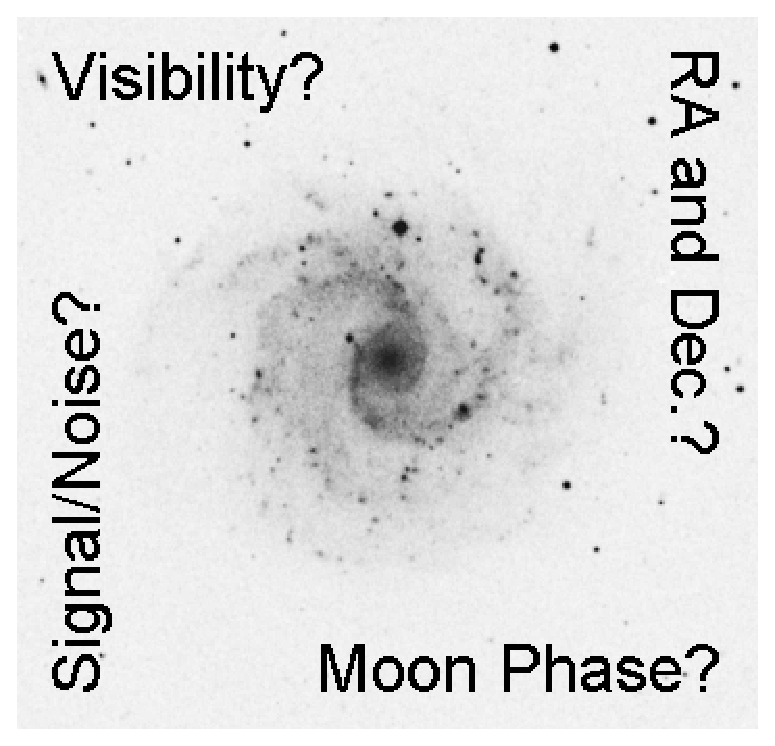
\includegraphics{sg10_front}
   \end{figure}
   \end{center}

% ? Headings.
   \begin{center}
      {\Large\bf Abstract}
   \end{center}

% ? End of heading for abstract.
\end{latexonly}

%  HTML documentation header.
%  ==========================
\begin{htmlonly}
   \xlabel{}
   \begin{rawhtml} <H1> \end{rawhtml}
      \stardoctitle
%      \stardocversion\\
%      \stardocmanual
   \begin{rawhtml} </H1> \end{rawhtml}

% ? Add picture here if required.
   \vspace{10mm}
   \begin{figure}[h]
   \leavevmode
   \centering 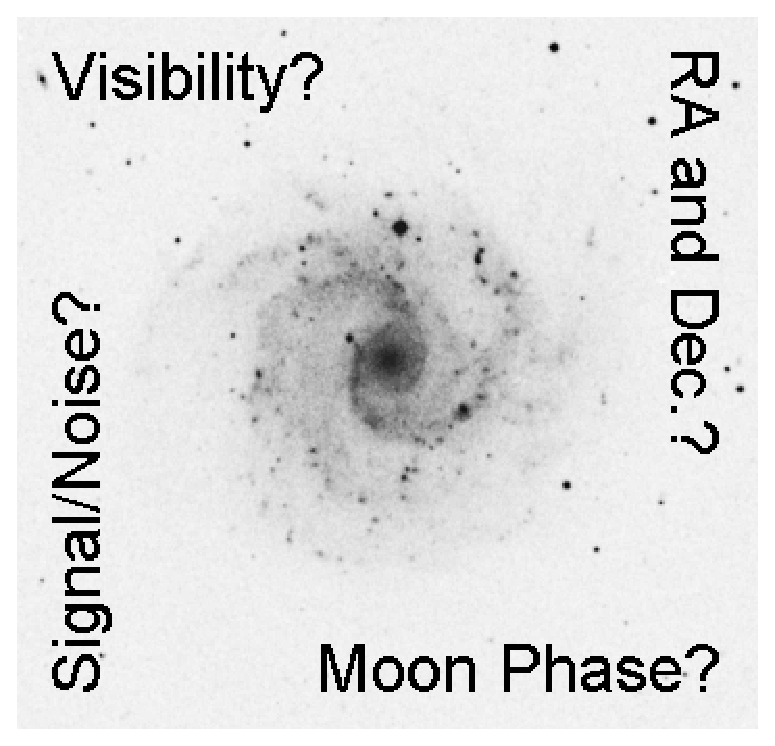
\includegraphics{sg10_front}
   \end{figure}
% ? End of picture.

   \begin{rawhtml} <P> <I> \end{rawhtml}
   \stardoccategory\ \stardocnumber \\
   \stardocauthors \\
   \stardocdate
   \begin{rawhtml} </I> </P> <H3> \end{rawhtml}
      \htmladdnormallink{CCLRC}{http://www.cclrc.ac.uk} /
      \htmladdnormallink{Rutherford Appleton Laboratory}
                        {http://www.cclrc.ac.uk/ral} \\
      \htmladdnormallink{Particle Physics \& Astronomy Research Council}
                        {http://www.pparc.ac.uk} \\
   \begin{rawhtml} </H3> <H2> \end{rawhtml}
      \htmladdnormallink{Starlink Project}{http://www.starlink.ac.uk/}
   \begin{rawhtml} </H2> \end{rawhtml}
   \htmladdnormallink{\htmladdimg{source.gif} Retrieve hardcopy}
      {http://www.starlink.ac.uk/cgi-bin/hcserver?\stardocsource}\\

%  HTML document table of contents.
%  ================================
%  Add table of contents header and a navigation button to return to this
%  point in the document (this should always go before the abstract \section).
  \label{stardoccontents}
  \begin{rawhtml}
    <HR>
    <H2>Contents</H2>
  \end{rawhtml}
  \newcommand{\latexonlytoc}[0]{}
  \htmladdtonavigation{\htmlref{\htmladdimg{contents_motif.gif}}
        {stardoccontents}}

% ? New section for abstract if used.
  \section{\xlabel{abstract}Abstract}
% ? End of new section for abstract
\end{htmlonly}

% -----------------------------------------------------------------------------
% ? Document Abstract. (if used)
%  ==================
\stardocabstract
% ? End of document abstract
% -----------------------------------------------------------------------------
% ? Latex document Table of Contents (if used).
%  ===========================================
 \newpage
 \begin{latexonly}
   \setlength{\parskip}{0mm}
   \latexonlytoc
   \setlength{\parskip}{\medskipamount}
   \markboth{\stardocname}{\stardocname}
 \end{latexonly}
% ? End of Latex document table of contents
% -----------------------------------------------------------------------------
\cleardoublepage
\renewcommand{\thepage}{\arabic{page}}

\setcounter{page}{1}

\section{Introduction} \xlabel{INTRODUCTION}
\label{sec:introduction}

One of the big problems with astronomy is that there are just not enough
telescopes go round. Most significant observatories and satellites are in use
virtually continuously, which means that competition
for observing time is very intense.

Aware of the precious nature of telescope time, many observers (and would be
observers) spend a lot of their time writing proposals requesting time, and
planning observations in an attempt to squeeze the maximum possible
information (and hence papers) out of a few brief nights atop some far flung
mountain or a few precious orbits of satellite time. In addition, if
time is awarded the ground-based applicant must then embark on the equally
intense effort required to obtain information (such as finder charts) that will
ensure that the run is success. Consequently, an enormous amount of work
must be undertaken to get to the stage where you have your
images/spectra/periodogram on a DAT or Exabyte tape. This time can be spent in a number of
ways which will include some of the following:

While writing your application:

\begin{itemize}
\item Identifying potential target objects. See \S{\ref{sec:cataloguem}} and \S{\ref{sec:catalogue}}.

\item Obtaining detailed up-to-date information on these objects. \S{\ref{sec:ads}}

\item Identifying the time of year at which the targets are accessible
      from a given site. See \S{\ref{sec:airmass}}.

\item Calculating the phase of the moon during the usable parts of the year. See
      \S{\ref{sec:airmass}}.

\item Determining if a specific observatory/satellite and its
      equipment is suitable for your purpose. See \S{\ref{sec:observatories}}.

\item Determining the exposures required to obtain
      a suitable signal/noise ratio for the proposed observation. See \S{\ref{sec:sn}}.

\end{itemize}

Then later when preparing for your observing run:

\begin{itemize}
\item Identifying other objects in the vicinity of the targets. See \S{\ref{sec:atlases}}.

\item Creating suitable finder charts. See \S{\ref{sec:finderc}}, \S{\ref{sec:catalogue}} and
      \S{\ref{sec:atlases}}.

\item Finding suitable objects for calibrating your observations. See \S{\ref{sec:catalogue}}.
\end{itemize}

For the PhD student or the inexperienced potential observer this amount of
work can be pretty daunting, requiring a steep learning curve between the
moment you had your bright idea for some observations and acquiring
the desired observations.

The aim of this document is to try to make life a little easier by
providing pointers to existing resources that are generally available
to users based at {\STARLINKref} nodes. It is anticipated that other
observers will also find some of the information useful.

\section{Resources} \xlabel{RESOURCES}
\label{sec:resources}

Having mentioned one of the bad things about astronomy, it's good to know that
there are nice things as well. One important thing to remember is that there
are an enormous number of resources available to the prospective observer and
that the number is increasing rapidly. When you hear older observers saying
``In my day we used to have to write the reduction software ourselves and wind
up the VAX every morning" they may not be exaggerating as much as you think.
For example, the RGASP package, and a number of others, was a direct result of
someone's PhD research programme.

The striking thing about this growth of resources is that they now appear in
many forms, including: software, books, web pages, and information provided by
the observatories.

It should not be forgotten that much useful information can be gained by
simply asking your colleagues what they use. This process will not always
identify the best, or even the most up-to-date resources, but it will at
least provide some sort of starting point from which you can look around for
others. A useful adage to get started with is ``If it works and you like it --
use it" but remember to keep your eyes open for better alternatives. It is
very easy to stay with a piece of software you are familiar with even when it
has long since been superseded by more modern, easier-to-use equivalents.

The sections that follow will identify examples from some of the
resource types mentioned above.


\subsection{The STARLINK Software Collection} \xlabel{STARLINK}
\label{sec:starlink}

One of the core activities of {\STARLINKref} is identifying
good software and making it available to the UK astronomical
community. The most visible manifestation of this
effort is the Starlink Software Collection ({\SSCref}) which is managed,
distributed and supported by the Starlink Project. A large amount of the
software was written by members of the Project, but some of it comes from
outside sources. Briefly put, it exists to provide the UK astronomy
community with the tools they need to get the job done.

By providing the software within a stable computing environment,
Starlink saves its users from the need to
acquire an in-depth knowledge of source code, compilers or linking. They
just sit down at a terminal and everything is virtually ready to go.

Clearly, at Starlink nodes the most important resource is the SSC
and you will find that most nodes have a large proportion of it installed.
However, if you find an item that you need is missing from your system,
just ask the system manager to add it.

The SSC is extensive, providing packages for a wide variety of purposes
including:

\begin{htmlonly}
\begin{itemize}
\item Image processing - {\KAPPAref}, {\ESPref}, {\DAOPHOTref}, {\PHOTOMref}, {\PISAref} and {\CCDPACKref}.)
\item Spectroscopy - {\DIPSOref}, {\ECHOMOPref}, {\FIGAROref} and
      {\SPECDREref}.
\item Time series analysis - {\PERIODref}
\item Polarimetry - {\POLMAPref} and {\TSPref}.
\item X-ray data processing - {\ASTERIXref}.
\item Millimetre wave band - {\SPECXref}.
\item Specific instruments - {\IRASref}, {\JCMTDRref}, {\IUEDRref} and {\CGSDRref}.
\item Image format conversion - {\CONVERTref}.
\item Graphics - MONGO, SM, {\PONGOref}).
\item Catalogue manipulation - {\CATPACref} and {\CURSAref}.
\end{itemize}
\end{htmlonly}
\begin{latexonly}
\begin{itemize}
\item Image processing -- KAPPA (SUN/95), ESP (SUN/180), DAOPHOT (SUN/42),
      PHOTOM (SUN/45), PISA (SUN/109) and CCDPACK (SUN/139).
\item Spectroscopy -- DIPSO (SUN/50), ECHOMOP (SUN/152), FIGARO (SUN/86) and SPECDRE (SUN/140).
\item Time series analysis -- PERIOD (SUN/169).
\item Polarimetry -- POLMAP (SUN/204) and TSP (SUN/66).
\item X-ray data processing -- ASTERIX (SUN/86).
\item Millimetre wave band -- SPECX (SUN/17).
\item Specific instruments -- IRAS90 (SUN/161), JCMTDR (SUN/132), IUEDR (SUN/37) and CGS4DR (SUN/27).
\item Image format conversion -- CONVERT (SUN/55).
\item Graphics -- MONGO (MUD/54), SM, PONGO (SUN/137).
\item Catalogue manipulation -- CURSA (SUN/190) and CATPAC (SUN/120).
\end{itemize}
\end{latexonly}

\subsection{{\STARLINKref} Software Collection -- Documentation} \xlabel{SSC}
\label{sec:ssc}

{\STARLINKref} software is documented in over 200 Starlink User Notes, hypertext
documents and the {\STARLINKWWWref} pages. Assistance is available
via email to {\tt starlink@jiscmail.ac.uk}.
A comprehensive description of the Starlink Software
Collection is available in Starlink document {\SUNONEref}. It can be
browsed on Starlink supported systems by typing ``{\tt showme sun1}" or via the
Starlink WWW pages at URL {\HTTPAref}

Getting information about a package is easy. If you want to find out the
name of Starlink documents relating to a piece of software (say
{\PISAref}) you need only type the following:

\begin{quote}
\begin{verbatim}
% docfind PISA
\end{verbatim}
\end{quote}

(where \% denotes the UNIX prompt) and the name of the document
will be displayed thus:

\begin{quote}
\begin{verbatim}
   Searching for the keyword pisa in the titles of documents ...

   SUN                    STARLINK USER NOTES                       SUN
   109.07  PISA - Position, intensity and shape analysis
\end{verbatim}
\end{quote}

Once you have that you will be able to display the document by typing:

\begin{quote}
\begin{verbatim}
% showme sun109
\end{verbatim}
\end{quote}

This will generate an Xmosaic or Netscape browser that will display
a WWW version of the document.

If the browser fails to appear, you can find the \LaTeX\ source of {\PISASUNref}
and all the other Starlink documents in directory ``{\tt /star/docs}".

\section{IRAF Too!} \xlabel{IRAF}
\label{sec:iraf}

As most of you are aware, the {\SSCref} (see \S{\ref{sec:ssc}}) is not a unique attempt to provide
a complete set of astronomical utilities and some {\STARLINKref} sites also have the
{\NOAOref} (National Optical Astronomical Observatories) supported {\IRAFref}
(Image Reduction and Analysis Facility) system installed alongside the home-grown SSC
items. IRAF is available as an item in the SSC but is written and updated
by NOAO. This is not true of the Starlink {\FIGAROref} which is directly maintained
by the Project.

The presence of both systems allows users to ``pick-and-mix" their
software usage (Starlink provides the image format conversion utilities
{\CONVERTref} to convert between the data formats used by the systems)
thereby obtaining the best of both worlds. In the context
of preparing to observe you will probably find the IRAF ASTUTIL (see \S{\ref{sec:astutil}})
and XEPHEM (see \S{\ref{sec:xephem}}) packages of most use.

Other systems ({\AIPSref}, {\MIDASref}, {\XANADUref}) may be available
at some nodes, but most install only the SSC and/or IRAF. Your system manager
will be able to advise you on what is available at your site.


\section{Software Packages and Utilities} \xlabel{PACKAGES}
\label{sec:packages}

A list of software packages commonly used while writing proposals is given
below under subject headings and then by program name. It is far from
exhaustive, but it does provide a basis from which to construct your own
set of favourite tools.

\subsection{Air mass/altitude/hour angle/visibility} \xlabel{AIRMASS}
\label{sec:airmass}

Once you have determined what it is that you intend to observe, the
next consideration is its visibility. If you are trying to observe
a source near the galactic centre in Sagittarius from La Palma, there is
little point in
applying for ground-based visible light telescope time in December, since
it will only be above the horizon during the day time. Similar
considerations apply to satellites, with applications attempting to image
within 50 or so degrees of the sun being dismissed. Consequently,
there is a plethora of programs that tell you how high an object is
(normally objects are only observed when less than 60 degrees from the
zenith) or when the object culminates.

Perhaps the easiest of these programs to use is {\OBSERVEref}
(see \S{\ref{sec:observe}}) which generates graphs and/or tables showing object
rise/set times. An example of the text and graphical output is shown in
the section describing OBSERVE. It is trivial to use and
can generate data for most the world's major observatories.

Those of you more familiar with IRAF may find you prefer to employ the
tools provided by the IRAF ASTUTIL utilities (see \S{\ref{sec:astutil}}).

If these do not provide exactly what you require, try SKYCAL (see \S{\ref{sec:skycal}}). While the
interface is rather clumsy, it does provide a lot of information.

\subsection{Bright/grey/dark time} \xlabel{BRIGHT}
\label{sec:bright}

As observers of very faint objects quickly come to realise,
the Moon is a real nuisance. If a bright Moon is present in the sky,
even at remote clean air sites, it scatters light across the whole sky
adding substantially to the sky background count and making really
faint objects increasingly difficult to observe. Because of this,
observations are broken up into targets requiring really dark skies,
those only needing fairly dark skies, and those where the
sky background is not important at all.

Those of you wanting to know about the Moon will find that the information is
available by using {\OBSERVEref} (see \S{\ref{sec:observe}}), with SKYCAL and
PREDICT (see \S{\ref{sec:skycal}} or \S{\ref{sec:predict}} respectively) offering
other sources of information.

\subsection{Binary-star predictions} \xlabel{BINARY}
\label{sec:binary}

Those of you interested in predictions of the phase of binary stars
will probably find what you want supplied by  the PREDICT package (see \S{\ref{sec:predict}}).

\subsection{Catalogue manipulation} \xlabel{CATALOGUEM}
\label{sec:cataloguem}

During the object selection phase you may want to take a catalogue of possible
objects and derive a subset with properties within range bounds you
have specified. This can be easily achieved using {\CURSAref} (see
SUN/190).

Using software like {\SKYCATref} (see \S{\ref{sec:skycat}})
it is also possible to view a FITS image
and overlay on the image the locations of objects identified from personal
catalogues.

Information on Internet sources of catalogue information may be found in \S{\ref{sec:catalogue}}.

\subsection{Co-ordinate system conversions} \xlabel{CORDS}
\label{sec:cords}

One of the perennial problems encountered in astronomy is the need to convert
between astronomical co-ordinate systems. The calculation of such transformations is tedious but
requires care. Probably the simplest way to avoid this problem is to use the
{\COCOref} package (see \S{\ref{sec:coco}}) which combines
a range of possibilities with a simple-to-use, no-nonsense interface.

Alternatively, you may care to try the ASTUTIL program GALACTIC (see \S{\ref{sec:galactic}}).


\subsection{Finder charts} \xlabel{FINDERC}
\label{sec:finderc}

Finder charts are an important tool for ground-based observing since
they give you the chance to examine the rest of the field and
identify nearby stars that may cause intrusive glare. This task can be performed
in two obvious ways:

\begin{itemize}
\item Use packages like {\CHARTref},
{\SKYMAPPCref} or {\SKYMAPUNIXref} (see \S{\ref{sec:skymappc}} and \S{\ref{sec:skymapsao}} respectively).

\item Download images of the region using on-line atlases
or finder charts created from the {\APMref} survey (see \S{\ref{sec:atlases}}).
\end{itemize}

The three packages named will all provide good finder charts.
You will find that {\SKYMAPPCref} is an IBM PC/Windows based package.
This has been included because it is very cheap, highly accurate and
self-installs.

The on-line atlas approach is dealt with in \S{\ref{sec:atlases}}.

\subsection{Signal/Noise} \xlabel{SN}
\label{sec:sn}

Calculating the time required to obtain a strong signal/noise detection
for a given object using a specific instrument usually requires an
in-depth knowledge of the instrument characteristics and other
parameters such as the local sky brightness. This calculation is probably
best undertaken using software supplied by the observatory in question, but
if that is not available the ASTUTIL CCDTIME program (see \S{\ref{sec:ccdtime}})
may be of some assistance. The
La Palma INT group supply two packages (see \S{\ref{sec:signal}}) dealing
with this problem.

\subsection{Ephemeris calculation} \xlabel{EPH}
\label{sec:eph}

For most purposes (no more accurate than an arcsecond or two) a satisfactory
planetary, lunar and solar ephemeris can be obtained using the FLUXES
package from Starlink.
However, if you wish to determine values more accurately you
would be well advised to access the JPL ephemeris using a couple of
simple SLALIB calls -- it really is very simple and is described fully
in {\JPLref} and {\SLALIBref}. Alternatively, you might care to try the {\SKYMAPPCref} or
XEPHEM packages (see \S{\ref{sec:skymappc}} and \S{\ref{sec:xephem}} respectively).

\section{Descriptions of Software Mentioned} \xlabel{DESOFT}
\label{sec:desoft}

The descriptions that follow borrow unashamedly from those provided by
the authors. This has been done to try to avoid inadvertently misrepresenting
the capabilities of any of the packages.

\subsection{ASTUTIL -- IRAF} \xlabel{ASTUTIL}
\label{sec:astutil}

This is an astronomical utilities package supplied by {\IRAFref}
as a layered package. It contains a number of useful programs of which the more
relevant are:

\subsubsection{AIR MASS}

Compute the air mass at a given elevation above horizon.

\subsubsection{ASTTIMES}

The astronomical quantities of universal time, J2000 Julian epoch, Julian
day, and local mean sidereal time at the specified observatory are computed
and printed for the given dates and times. The input dates and times may be
taken from files containing the year, month, day, and local time in the
specified time zone or, if no files are specified, then task parameters are
used.  The output consists of a printed table with optional header, a copy of
the input data, and derived astronomical data.

\subsubsection{CCDTIME} \xlabel{CCDTIME}
\label{sec:ccdtime}

A telescope, CCD detector, and list of filters is selected from a database to
define the expected photon/electron count rates.  These rates, along with a
specified seeing and air mass, are used to estimate the signal-to-noise ratio
for a stellar observation in each filter.  The output provides three
results per filter: the exposure time to achieve a desired signal-to-noise
ratio for a given magnitude, the magnitude to achieve a desired
signal-to-noise ratio in a given time, and the signal-to-noise ratio
at a specified magnitude and exposure time.

\subsubsection{GALACTIC} \xlabel{GALACTIC}
\label{sec:galactic}

GALACTIC is used to convert between equatorial and galactic coordinates or
vice versa. Co-ordinates are read from the input file as Right Ascension and Declination or
galactic longitude and latitude pairs. Each co-ordinate pair may optionally be
followed by the epoch of the equatorial co-ordinates, in which case the
co-ordinates are precessed to 1950.0 before conversion for equatorial to
galactic or to the specified epoch for galactic to equatorial.

\subsubsection{PRECESS}

Co-ordinates are read from the input file as Right Ascension and Declination pairs, one pair per
input line.  Each co-ordinate pair may optionally be followed by the equinox
of the input co-ordinates (if different from the default) and the epoch of the
output co-ordinates.  Co-ordinates may be entered in either decimal or
sexagesimal notation.  The given co-ordinates are rotated according to the
precession rates to the requested year and printed on the standard output.
Basic data is taken from the Explanation to the American Ephemeris.


\subsection{{\CURSAref} -- {\STARLINKref}} \xlabel{CURSA}
\label{sec:cursa}


{\CURSAref} is a set of {\STARLINKref} programs for manipulating astronomical
catalogues and similar tabular datasets. It provides facilities for: browsing
or examining catalogues, selecting subsets from a catalogue, sorting
catalogues, copying catalogues and pairing two catalogues. Subsets can be
extracted from a catalogue in a format suitable for plotting using other
Starlink packages, such as {\PONGOref} (see {\PONGSUNref)}. CURSA can access
catalogues held in the popular FITS table format, as ASCII text, or in the
CHI/HDS format used by the {\CATPACref} catalogue manipulating programs.

CURSA will also handle small(ish) catalogues or private tables of the user's
favourite objects, selecting those objects which match the constraints of a given
observing programme.

\subsection{{\CHARTref} -- {\STARLINKref}} \xlabel{CHART}
\label{sec:chart}

\begin{figure}[htbp]
\leavevmode
\centering 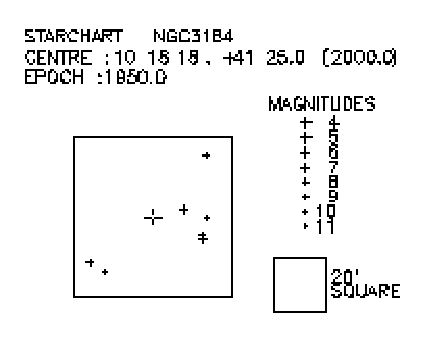
\includegraphics{sg10_chart}
\vspace{5mm}
\caption{Example CHART output.}
\label{fig_chart}
\xlabel{fig_chart}
\end{figure}

The {\CHARTref} package extracts positions, magnitudes and other data from certain
stellar and non-stellar astronomical catalogues. The results may be listed on
a terminal or printer, or used to plot finding charts or perform astrometric
reductions.

An example of the graphical output is shown in Figure 1.
The stars may be identified via
a text table supplied by the program. An example would be something like:

{\scriptsize
\begin{quote}
\begin{verbatim}
 Input Field Centre  10 18 18.000    + 41 24 58.00  Equinox 2000.00
    Equivalent to  10 15 18.554    + 41 40  0.14  Equinox 1950.00

    Galactic Coordinates:            b  =  55.64      l  = 178.35
    Ecliptic Coordinates (1950.00):Lat. =  28.61   Long. = 139.79

       Output positions for Equinox 1950.00    Epoch 1950.00

       ******************************************************
       * Approximate Field Centre Location on Sky Survey(s) *
       ******************************************************
           Survey      Field Centre          X        Y
           Palomar     +42  10H  0M          82      187

             Number of CSI Catalogue stars found =  25
    HD          DM       Spec   V      B         R.A.       Dec.        Offsets
                               Mag   Mag           (1950.00)           From Centre
                                                                          "       "     Idents
1  88513   BD +42  2100   F2   8.2   8.6     10 10 27.1   +42  7 52    -3242   1695    AGK,SAO
2  88577   BD +42  2102   G5   8.4   9.8     10 10 51.7   +42  3 45    -2972   1444    AGK,SAO
3          BD +42  2103   K2 ( 9.5) 10.7     10 11 23.3   +42 20 31    -2609   2446    AGK,SAO
4  88785   BD +42  2104   F2   8.2   8.6     10 12 25.6   +42  7 26    -1924   1654    AGK,GCRV
5          ** +42 10124   K0 (10.8) 12.0     10 12 28.7   +42 38  7    -1875   3495    AGK
\end{verbatim}
\end{quote}
}

The following catalogues are available within CHART.

\subsubsection{CSI}

Stars can be selected from the Catalogue of Stellar Identifications (CSI)
1979 edition, prepared by the ``Centre de Donnees astronomiques de
Strasbourg" (CDS). This is a
compilation of 434,927 stars, extracted from a wide range of original source
catalogues. Approximate positions are available for each star, together with
cross references into the original source catalogues. Magnitudes are
available for most of the stars. Used in this mode, the program can act as a
stellar data retrieval system to find, for example, which stars are (or are
not) in a particular catalogue, or what information is known about the stars
in a particular field. This is also the normal mode of use when preparing
overlays or finding charts.

\subsubsection{Astrometric}

Stars can be selected from a merged astrometric catalogue (prepared at {\RGOref} by
W.~Nicholson). This contains the whole of the AGK3 catalogue (extending down
to Dec -3 degrees), the SAO stars south of the celestial equator, and the complete
PERTH70 catalogue. This catalogue contains fewer stars than the CSI
catalogue, but includes accurate positions and proper motions as well as
magnitudes and spectral types. This mode is most useful when preparing to
carry out astrometry.

\subsubsection{Non-Stellar}

Nonstellar objects can be selected from the Dixon `Master List of Nonstellar
Objects'. This was formed by a simple merging of many catalogues and lists.
The total number is about 185,000. Approximate angular sizes and magnitudes
are given for many objects.

\subsubsection{Private}

Stars can be selected from any catalogue that has been produced in the form
that {\CHARTref} expects for `ASTROMETRIC' mode.

You can select which of these four modes to work in and specify a series of
search areas. In CSI, ASTROMETRIC or PRIVATE modes you can also place
magnitude or total number limits on the search and choose which source
catalogues to include or exclude. A series of field centres may be input at
the terminal or read from a previously prepared file.

After the search is made, you may list the results at a terminal or on the
printer. Positional information may be precessed to a specified equinox.

You may also plot the results in the form of an overlay or finding chart.


\subsection{{\COCOref} -- {\STARLINKref}} \xlabel{COCO}
\label{sec:coco}


The {\COCOref} program converts star co-ordinates from one system to another.  Both
the improved IAU system, post-1976, and the old pre-1976 system are
supported. COCO can perform accurate transformations between the following
co-ordinate systems:

\begin{itemize}
\item mean RA and Dec., old system, with E-terms (loosely FK4, usually B1950)
\item mean RA and Dec., old system, no E-terms (some radio positions)
\item mean RA and Dec., new system (loosely FK5, usually J2000)
\item geocentric apparent RA and Dec., new system
\item ecliptic co-ordinates $[\lambda,\beta\,]$, new system (mean of date)
\item galactic co-ordinates $[l^{II},b^{II}]$, IAU 1958 system
\end{itemize}

{\COCOref}'s user-interface is spartan but efficient.  The program offers control
over report resolution, and has a simple online help facility. All
input is free-format, and defaults are provided where this is meaningful.

The input/output arrangements of COCO are flexible, to allow a variety of
operating styles -- interactive, input from a file, report to a file, batch,
{\it etc}. Also, in addition to the report which is produced, the results of
the conversions are also available in a raw form, to a fixed resolution and
free from extraneous formatting.
This file is intended to be read easily by other programs.

In order to comply with the IAU 1976 recommendations, all position data
published from 1984 on should be given in the new system, using equinox
J2000.0. However, positions are still frequently given in the old system,
using equinox B1950.0. COCO can perform the necessary conversion.


\subsection{{\OBSERVEref} -- {\STARLINKref}} \xlabel{OBSERVE}
\label{sec:observe}

The program {\OBSERVEref} is designed to allow you to get a quick overview
of the observability of a star through the year from the geographical
location selected. You will be prompted for the Right Ascension and Declination
of the star/object, the telescope employed, and the year. On the selected
graphics device a
plot will be drawn that tells you, for all dates of the year, the star rising
and setting times and the times that it is 30 degrees above the horizon
(air mass less than 2), the
times of astronomical twilight, the phase and rising and setting times of the
Moon as well as its distance from the star in question.

The algorithms used in calculating these times, positions and phases come
from the book `Practical Astronomy with your calculator' by
P.~Duffett-Smith (3$^{\rm rd}$ ed.~CUP 1988), and are used with permission.
These algorithms are not designed for very high precision calculations, a
fact which is to some extent conveyed by the program output. Nevertheless,
it has been verified that the routines are good for their purpose.
As mentioned above, all standard Starlink graphics devices are supported.
The data generated by {\OBSERVEref} can also be output to a text file.

\begin{figure}[htbp]
\leavevmode
\centering 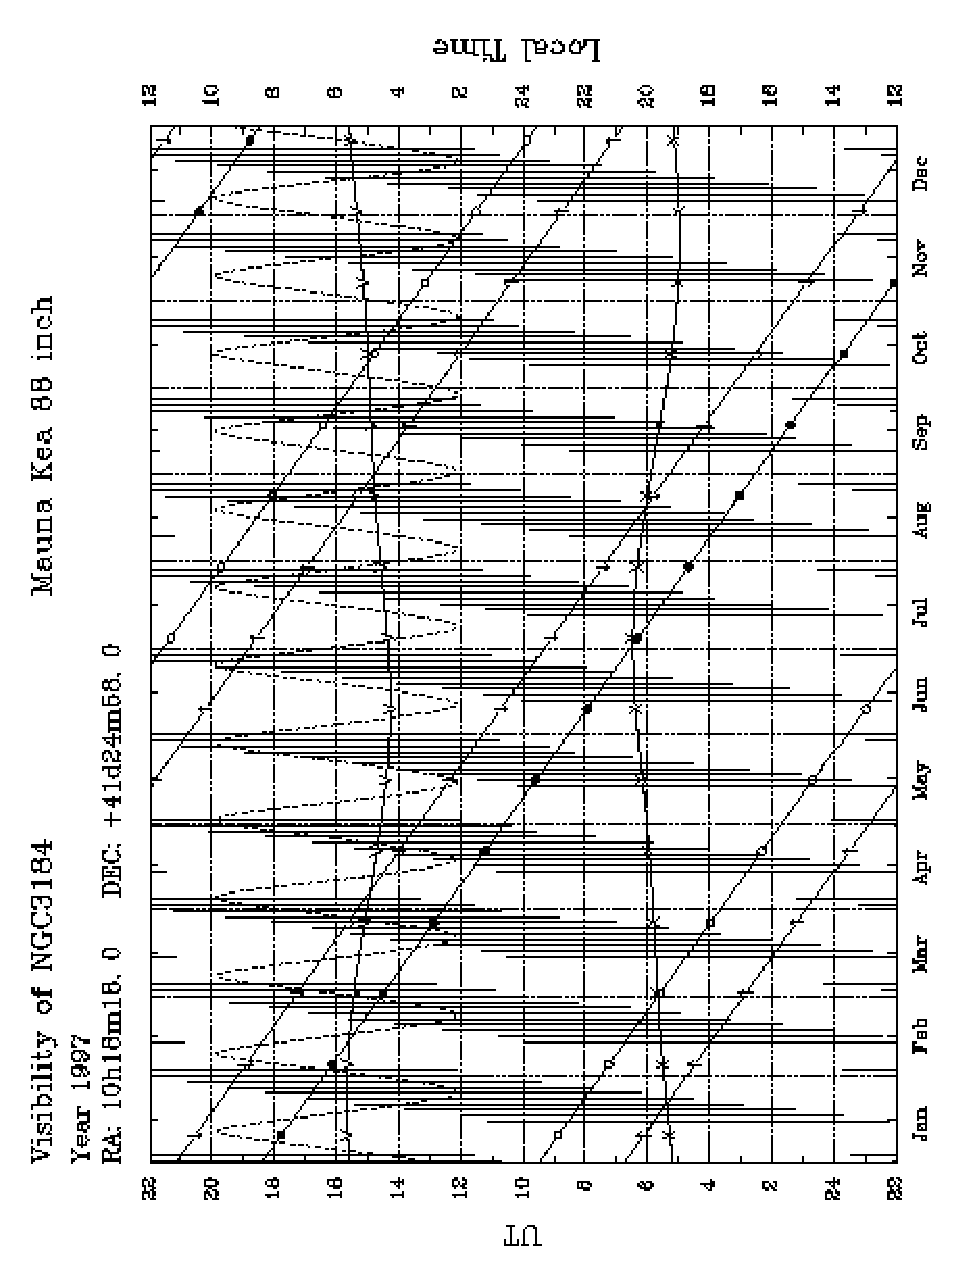
\includegraphics{sg10_obs}
\caption{Example OBSERVE output.}
\end{figure}

The format of the text file is shown below:
{\scriptsize
\begin{quote}
\begin{verbatim}
Object selected was: NGC3184

Located at RA:       10h18m18. 0
Located at Dec:      +41d24m58. 0

From:                Mauna Kea 88 inch
During:              1997

January

Day    Rise    Set      Above 30 Below 30  Twi. beg Twi end   Moon ris Moon set Moon dist  Moon %
01   06:42:10 21:08:09  09:27:53 18:22:26  15:35:46 05:11:31  10:43:52 22:08:22 15:07:03     60
02   06:38:14 21:04:13  09:23:57 18:18:30  15:36:08 05:12:05  11:34:52 22:47:07 15:42:22     51
03   06:34:18 21:00:17  09:20:01 18:14:34  15:36:29 05:12:38  11:35:28 23:28:06 16:21:27     41
04   06:30:22 20:56:21  09:16:05 18:10:38  15:36:50 05:13:12  12:28:57 00:12:20 17:03:24     31
05   06:26:26 20:52:25  09:12:09 18:06:42  15:37:10 05:13:46  13:24:50 01:00:45 17:47:37     22
\end{verbatim}
\end{quote}
}

\subsection{PREDICT -- RGO} \xlabel{PREDICT}
\label{sec:predict}

Predict was designed for those observers wishing to get data on binary stars
in particular. It gives data for the Moon and programme stars in the form of
a listing for every 15 minutes from the end of evening nautical twilight to
the start of morning nautical twilight. This listing would include orbital
phase, given a time of minimum and period for the programme star, its
altitude, azimuth, air mass and angular separation from the moon. Times of
twilight are calculated as well as moonrise/set object rise/set. A simple
phase diagram showing the observable phase can also be produced.  At the
moment it runs on a VAX, but it is being ported to the Linux system and upgraded
with more accurate Sun/Moon algorithms.


\subsection{SKYCAL -- John Thorstensen} \xlabel{SKYCAL}
\label{sec:skycal}

This consists of two programs, SKYCALC and SKYCALENDAR.

SKYCALC is an "Interactive Almanac." It helps you plan and execute observing
runs, and allows easy calculation of air masses, twilight, lunar interference,
co-ordinate transformations and such -- nearly everything except the weather.

SKYCALENDAR is a "Nighttime Astronomical Calendar" to calculate and
print astronomical calendars.

Both programs have several preset Observatory locations to choose from.
You can also specify your own.

A copy of the SKYCAL code can be obtained via Starlink, together with the
document {\SUNSKYref}.

\subsection{{\SKYCATref} -- ESO}  \xlabel{SKYCAT}
\label{sec:skycat}

{\SKYCATref} allows you to open and visualise a variety of FITS images including
support for World Co-ordinate System (WCS), interactive measurement of offsets,
and other standard visualization functions (SAOimage-like). It is possible to
access and load an image from a network server of the Digitized Sky Survey
scans and access catalogue information from a number of popular astronomical
catalogues like the ``HST Guide Star Catalog" (GSC) and others.

It is also possible to access the observations catalogue from the NTT, HST and
CFHT Science Archives, and use {SIMBADref} or {\NEDref} both as name resolvers as well as
for information on known objects.


\subsection{SKYMAP -- SAO} \xlabel{SKYMAPSAO}
\label{sec:skymapsao}

SKYMAP is a sophisticated interactive display program which can be used to
create finder charts at any particular plate scale.
The package can plot any
two catalogues from its list, plus stars from the {\GSCref}. The planetary positions
are taken from the current JPL ephemeris.

All-sky maps can also be produced to show large structures or
the position of a catalogue in the big picture. All of the IRAS plate projections
 are included so objects can be plotted
against contoured IR sky flux. Catalogue objects may be identified by
plotting a catalogue over an image.

The package runs on Tektronix-compatible devices and is fairly sophisticated.


\subsection{{\SKYMAPPCref} -- Chris Marriott} \xlabel{SKYMAPPC}
\label{sec:skymappc}

This versatile PC-based package allows you to create finder charts showing
the area around your target object and all stars in the {\GSCref} and SAO
catalogues together with objects from the NGC and IC catalogues overlaid.

{\SKYMAPPCref} is available from it's own home page at
URL {\HTTPCref}. Versions exist for Windows, Windows NT and Windows 95.
The software is inexpensive shareware (\pounds 30) at the time
of writing. It runs best on 386s (or better CPUs) with more than 4Mb of RAM
available.


\subsubsection{Stars}

The 1990 machine-readable version of the SAO star catalogue is the source of
star data. The evaluation version of {\SKYMAPPCref} comes with stars to magnitude 7;
the commercial version of the program is supplied with the complete SAO
catalogue of stars -- this is reasonably complete down to magnitude 9.5.

The commercial version of {\SKYMAPPCref} can also display stars (and other objects)
read from the {\GSCref} CD-ROM database.

\subsubsection{Solar system}

The positions of the planets Mercury to Pluto plus the Sun and Moon are
shown, with a mean error of less than an arcsecond. The Moon is drawn with
the correct phase and orientation in the sky. Clicking on any planet displays
extensive positional and physical information (position, distance, phase,
visual magnitude, light time, etc). Planetary positions are rigorously
reduced for the topocentric position of the observer.
The program is supplied with a catalogue of asteroids and comets.

\subsubsection{Galaxies etc}

{\SKYMAPPCref} is supplied with the complete Saguaro Astronomy Club (SAC) v6 database
of 10,700 deep sky objects. This contains the complete Messier, Revised NGC, and IC
catalogues, together with the brighter objects from more than 80 other object
catalogues. Extensive information about any object can be displayed.

\subsection{XEPHEM -- {\IRAFref}}   \xlabel{XEPHEM}
\label{sec:xephem}

XEPHEM version 2.6 is an interactive astronomical ephemeris program for X
Windows systems. It computes heliocentric, geocentric and topocentric
information for celestial objects. It has built-in support for all
planets: the moons of Jupiter, Saturn and Earth, and Mars' central meridian
longitude. Xephem supports objects in heliocentric or Earth orbit, given the
appropriate elements. Sample databases of over 16000 objects are included in
the release kit.

XEPHEM generates data in configurable tabular forms and in several detailed
graphical formats. It can plot and list all data fields and can be
programmed to search for arbitrary circumstances.


\section{Observatories} \xlabel{OBSERVATORIES}
\label{sec:observatories}


Usually, the best place to look for information on the capabilities of the
instruments and telescopes at an observatory is in the Web pages of
the observatory that operates it. The URLs of some the observatories
used by British observers:

\begin{itemize}
\item Anglo-Australian Observatory -- {\HTTPGref}
\item AAT 2DF -- {HTTPBCref}
\item CFHT -- {\HTTPBZref}
\item Royal Observatory Edinburgh -- {\HTTPHref}
\item Royal Greenwich Observatory -- {\HTTPIref}
\item ING La Palma (WHT/INT/JKT) -- {\HTTPJref}
\item ING Software -- {\HTTPJref}
\item JAC Hawaii (UKIRT/JCMT) -- {\HTTPKref}
\item JAC Software -- {\HTTPLref}
\item SAAO -- {\HTTPBAref}
\item MERLIN -- {\HTTPBBref}
\end {itemize}

\subsection{SIGNAL and LIGHT\_IN\_SLIT} \xlabel{SIGNAL}
\label{sec:signal}
Those of you interested in using instruments at La Palma will find the SIGNAL and
LIGHT\_IN\_SLIT packages provided by Chris Benn particularly useful.

\subsubsection{SIGNAL}

SIGNAL is a Fortran program for predicting the number of object and sky
photons detected during an exposure with one of the common-user instruments
of the Isaac Newton Group telescopes. The predictions are based on a
combination of measured and estimated efficiencies for the telescopes,
cameras, gratings and detectors.

\subsubsection{LIGHT\_IN\_ SLIT}

LIGHT\_IN\_SLIT calculates the refractive index at each wavelength for an
arbitrary atmosphere, and uses this to calculate wavelength-dependent total of
light entering slit (at arbitrary angle on sky) from a circularly symmetric
Gaussian image at arbitrary zenith angle.

Copies of the current versions (for SUN workstations) are available
from URL:
\begin{quote}
{\tt ftp://ftp.ast.cam.ac.uk/pub/pubinfo/signal/}
\end{quote}

\section{FORMLOAD} \xlabel{FORMLOAD}
\label{sec:formload}

As many of you are aware, applications for observing time on
telescopes such as the AAT, INT or WHT must be submitted to the
selection process in the proper format. The forms involved (such as PATT2)
are quite complex and compactly laid out. They can be filled out by careful
use of a typewriter (if you can still find such a thing) but are most
conveniently filled out using a Starlink package named FORMLOAD, which was
designed for the purpose.

The user of the package has to prepare a text file which provides the
information that is embedded in the appropriate parts of the final
application form. To make this easier, template files are provided for each
of the forms. The associated document {\SUNFORMref} provides information
on the details of the process.

Support is provided for:

\begin{itemize}
\item UK optical and infrared telescopes (PATT2).
\item La Palma ING telescopes scheduling information.
\item UK millimetre and submillimetre telescopes (PATT3).
\item AAT telescopes scheduling.
\end{itemize}

The software runs under UNIX and VMS.

\section{On-line Atlases -- Finder Charts} \xlabel{ATLASES}
\label{sec:atlases}

One of the best ways to make a finder chart is by the use of an on-line
atlas, the most famous of which are those provided by NASA, ESO and the STScI.
They are very simple to use. You supply the Right Ascension and Declination values for the region
of sky you are interested in, specify the dimensions of the chunk of
sky you wish to examine, and the WWW site sends you an appropriate FITS or GIF
file. The whole procedure takes about 3 minutes.

The image requested is supplied
from a database containing the entire sky as generated by digitally sampling
scans of Palomar, UK or ESO Schmidt survey plates. The resolution and accuracy of the data may
vary slightly depending on the source of the plates employed and the scanner
they were sampled with.

URLs for the four most popular on-line atlases are given below:

\begin{itemize}
\item CADC -- {\CADCref}
\item ESO -- {\HTTPEref}
\item Skyview -- {\HTTPDref}
\item STScI -- {\HTTPFref}
\end{itemize}

An example of the quality of output can be seen on the front cover of this document.
The image of NGC3184 was supplied by Skyview in its default setting.

Some of the sites also allow catalogue overlays onto the images provided
(so that nearby objects can be readily identified)
and co-ordinate/name resolution.
You give the name (say) NGC4395 and
it gives back the co-ordinates  RA 12 25 53.0  Dec.\ 33 32 54 which it
then employs as the target location.

Alternatively, you may be at a site that possesses the ``Digitised
Sky Survey" (supplied in the form of 102 CD-ROMs) or the more highly compressed
``RealSky" (9 CD-ROMs). You will find that these come with software which
allows you to choose a chunk of sky to look at, tells you which CD to place in
the CD-ROM player, and then creates the image for you.

The {\APMref} Sky Catalogue also contains information gained from scanned survey plates, but
stored in the form of a description database rather than as images. It is used in a very similar manner to the atlases.
You go to the appropriate URL and after entering the co-ordinates, epoch and field size
are provided with maps (B and R band) showing the locations of all objects detected in that field.
The maps are provided as GIFs or Postscript files, together with a text file describing each object.
The appearance of the maps is tidy, simple and uncluttered.

The APM survey can be found at:

{\tt
\begin{quote}
\begin{verbatim}
http://www.ast.cam.ac.uk/~rgm/apm_catalogues.html
\end{verbatim}
\end{quote}
}

\section{Books and Plates} \xlabel{BOOKS}
\label{sec:books}

In the rush to power-up your workstation and get a Web browser
running, do not forget that other long established sources of information
exist and can probably be found in your departmental library.
For example:

\begin{itemize}
\item The British Astronomical Association Handbook.
A source of much information,
particularly pertaining to objects in the solar system, with some useful tables and
information about time and time signals.
\item Norton's 2000 Star Atlas and Reference Handbook, Editor Ian Ridpath, Longman Scientific,
ISBN 0-582-03163-X. A good entry-level guide to the sky and observing.
\item Uranometria, Will Tirion. A more complete atlas showing stars down to 10th
magnitude and galaxies/nebulae considerably fainter.
\item Nautical Almanac, HM Nautical Almanac Office, HMSO.
\item Schmidt Survey Plate copies. Copies of the original plates on which
the digitised sky surveys are based.
\end{itemize}


\section{Internet Sources for the Software Described} \xlabel{SOURCESSOFT}
\label{sec:sourcessoft}

A list of useful URLs is provided below, but some links may (as seems to be
the way on the Web) be subject to change without notice. If you find any
failing please tell us.

\begin{itemize}
\item ASTUTIL -- {\HTTPBref}
\item CURSA --  {\HTTPBDref}
\item CHART -- {\HTTPBEref}
\item COCO -- {\HTTPAref}
\item OBSERVE -- {\HTTPAref}
\item PREDICT -- Via Steve Bell. Email {\tt sab@ast.cam.ac.uk}
\item SKYCAL -- {\HTTPAref}
\item SKYCAT -- {\HTTPMref}
\item SKYMAP (PC) -- {\HTTPCref}
\item SKYMAP (UNIX) -- {\HTTPNref}
\item XEPHEM -- {\HTTPBref}
\end{itemize}

It is worth bearing in mind that the {\IRAFref} Web site is now mirrored
in the UK at:
\begin{quote}
{\tt http://www.starlink.ac.uk/iraf/}
\end{quote}
allowing the complete binaries to be downloaded in just a few minutes.

The STScI also maintain a very useful directory of astronomical software at:

\begin{itemize}
\item ASDS (STScI Astronomical Software Directory) -- {\HTTPOref}
\end{itemize}

\section{Internet Catalogues and Databases} \xlabel{CATALOGUE}
\label{sec:catalogue}

If you are interested in looking at on-line astronomical databases you
will find that the Starlink documents {\SUNCATref} and {\SUNCATBref} provide a very full account.
Some portions of SUN/162 are, inevitably, a little out-of-date, but much of the information
it contains is still very useful. Another source of information is
the ``Network Resources for Astronomers" site at URL
{\HTTPBFref}.

However, to allow you to quickly examine some of the most popular databases, some
URL are given below:

\begin{itemize}
\item APS -- {\HTTPPref}
\item CDS -- {\HTTPQref}
\item CIO -- {\HTTPRref}
\item NASA ADS -- {\HTTPSref}
\item NASA NED -- {\HTTPTref}
\item SIMBAD (Europe) -- {\HTTPUref}
\item SIMBAD (USA) -- {\HTTPVref}
\end{itemize}

Descriptions of the databases and catalogues are given in the next section.

\subsubsection{APS image database} \xlabel{APS}
\label{sec:aps}

The APS Catalogue of the POSS I is the result of scans of glass duplicates of
the blue (O) and red (E) plates of the original Palomar Observatory Sky
Survey (POSS I) for 664 fields.

The object Catalogue entries include images, calibrated magnitudes in two
colours, positions to 0.2 arcseconds and neural network image
classifications.

\subsubsection{CDS} \xlabel{CDS}
\label{sec:cds}

The ``Centre de Donnees astronomiques de Strasbourg" (CDS) collects and distributes
astronomical data catalogues, related to observations of stars and galaxies,
and other galactic and extragalactic objects. A few catalogues about the
solar system bodies and atomic data are also included.

Importantly, this site hold copies of three papers by Landolt describing standard
stars in the UBVRI wavelength bands.

The catalogues and tables managed by CDS can be summarized as follows:

\begin{itemize}
\item  More than 1700 Catalogues available from CDS.
\item  More than 1290 are available on-line (as full ASCII or FITS files).
\item  More than 1090 are also available through the VizieR browser.
\end{itemize}

\subsubsection{CIO} \xlabel{CIO}
\label{sec:cio}

The Catalogue of Infrared Observations is a database of over 200,000
published infrared observations of more than 10,000 individual astronomical
sources over the wavelength range from 1 to 1000 micron. The catalogue is
available for downloading via ftp.

\subsubsection{NASA {\ADSref}} \xlabel{ADS}
\label{sec:ads}

The Astrophysics Data System ({\ADSref}) is a resource that provides
astronomical data to the scientific user community. At present the main
emphasis is on the Abstract Service, which includes three sets of abstracts:

\begin{itemize}
\item Astronomy and astrophysics, containing approximately 240,000 abstracts.
\item Space instrumentation, containing approximately 410,000 abstracts.
\item Physics and geophysics, containing approximately 220,000 abstracts.
\end{itemize}

The abstracts contain information on papers published in a number of refereed
scientific publications. This should not be confused with databases that contain
information derived from publications such as redshift or luminosity.
Each dataset can be searched by author, object name, title, or abstract text
words. In addition, the abstracts include links to scanned images of over
20,000 journal articles appearing in `Astronomy and Astrophysics',
 `ApJL' and `AJ' since 1975, `ApJ'
since 1990, and `PASP' since 1988.

In addition to the Abstract Service, the {\ADSref} provides access or pointers to
NASA data catalogues and data archives, thereby making data collected by NASA
missions available to astronomers.

\subsubsection{NASA Extragalactic Database -- {\NEDref}/IPAC} \xlabel{NED}
\label{sec:ned}

The NASA/IPAC Extragalactic Database ({\NEDref}) is built around a master list of
extragalactic objects for which cross-identifications of names have been
established, accurate positions and redshifts entered to the extent possible,
and some basic data collected. Bibliographic references relevant to
individual objects have been compiled, and abstracts of extragalactic
interest are kept on line.

The most recently updated version of the NED database contains positions,
basic data, and over 710,000 names for 375,000 extragalactic objects, as well
as nearly 625,000 bibliographic references to 27,000 published papers, and
35,000 notes from catalogues and other publications. NED supports searches for
objects and references, and offers browsing capabilities for more than 11,400
abstracts of articles of extragalactic interest that have appeared in
Astronomy and Astrophysics, AJ, ApJ, MNRAS, and PASP since 1988, and in
Publications of the Astronomical Society of Japan, Astronomy Reports and
Astronomy Letters (formerly Soviet Astronomy and Soviet Astronomy Letters)
since 1992.

Over 645,000 detailed photometric measurements, and 250,000 detailed position
measurements, taken from catalogues and the published literature, are currently
available through NED. Also on-line are selected IAU Circulars as well as
thesis abstracts of doctoral dissertations on extragalactic topics. Title and
abstract searches of the NED literature database can now be made by
specifying author names. It is also possible to search the main NED database
for objects selected by redshift ({\NEDref} currently has over 45,000 velocities),
in addition to the selection by name, by position, or by type.

\subsubsection{{\SIMBADref}} \xlabel{SIMBAD}
\label{sec:simbad}

The {\SIMBADref} astronomical database, created and maintained by the CDS,
Strasbourg, brings together basic data, cross-identifications, observational
measurements, and bibliography, for celestial objects outside the solar
system: stars, galaxies, and nonstellar objects within our galaxy, or in
external galaxies. In total, SIMBAD contains data for roughly
1,000,000 objects.

In some instances there is a charge for using SIMBAD, so a password may be needed.
However, the charge is paid by the ESA for institutions in member states. Most
{\STARLINKref} sites will probably already have a password. Your site manager
should be able to advise you on this.

A mirror site exists in the USA.

\section{Internet Links to Astronomical Resources} \xlabel{LINKS}
\label{sec:links}

When it comes to searching for a variety of resources the URLs below
are pretty hard to beat. They are well maintained and provide a huge amount
of information.

\begin{itemize}
\item NRAO  Astronomy on the Web -- {\HTTPWref}
\item NRAO Astronomy Software Servers -- {\HTTPYref}
\item STScI Astronomical Resources -- {\HTTPXref}
\item STScI Astronomical Software Directory  -- {\HTTPZref}
\item AstroWeb -- {\HTTPBGref}
\end{itemize}

\section{Internet Software Archives} \xlabel{GENERAL}
\label{sec:general}

The sites listed below contain an enormous number of software packages (most
of them non-astronomical). They are particularly well suited to finding
planetarium software and databases.

\begin{itemize}
\item Imperial College Sunsite -- {\HTTPAAref}
\item HENSA (PC) -- {\HTTPABref}
\item HENSA (UNIX) -- {\HTTPACref}
\item Oakland VSL -- {\HTTPADref}
\end{itemize}

\section{Acknowledgments} \xlabel{ACK}
\label{sec:ack}

I would like to acknowledge the assistance of Mike Lawden, Peter Draper and
Clive Davenhall who pointed out most of the places I went wrong
in the first draft of this document.

\vspace{3cm}

\subsection*{Revision History}

\begin{enumerate}

  \item 18 March 1997: Version 1 (GJP).

  \item 30 January 1998: Version 2.  Corrected the reference to CURSA
   in Section 4.4, {\it Catalogue manipulation\/} (ACD).

\end{enumerate}


\end{document}

